\documentclass[11pt]{article}
\usepackage[margin=1in]{geometry}
\usepackage{graphicx}
\usepackage{booktabs}
\usepackage{hyperref}
\usepackage{natbib}
\usepackage{amsmath}
\usepackage{amssymb}
\usepackage{textcomp}
\usepackage{tabularx}
\usepackage{microtype}
\usepackage{setspace}
\hypersetup{colorlinks=true, linkcolor=black, citecolor=black, urlcolor=blue}

\title{Sentiment Analysis of Letterboxd Movie Reviews:\\
A Classical NLP Baseline Study}
\author{Nikolai Tristan Pazon\\Heart Alvern Sumicad\\Jade De Paz}
\date{\today}

\begin{document}
\maketitle

\onehalfspacing

\begin{abstract}
\noindent We investigate whether a fully classical NLP pipeline can recover the sentiment of Letterboxd movie reviews from text alone. After cleaning the public Kaggle export from 90{,}016 raw rows down to 3{,}376 deduplicated, balanced reviews, we train four pipelines built from TF-IDF and bag-of-words features. The strongest classifier is multinomial Na\"ive Bayes on TF-IDF unigrams and bigrams: \textbf{accuracy 0.852}, \textbf{macro F1 0.852}, and \textbf{ROC AUC 0.917} on the held-out test split. The result echoes long-standing observations on text classification with simple linear models~\citep{joachims_1998, mccallum_nigam_1998, wang_manning_2012}. We document each step of the pipeline, justify our choices against the literature, and analyse the residual errors.
\end{abstract}

\section{Introduction}

Sentiment analysis is one of the most heavily studied tasks in natural language processing. The seminal large-scale study by~\citet{pang_lee_vaithyanathan_2002} showed almost twenty-five years ago that movie reviews are a particularly attractive target: the prose is informal, the supervision signal (a star rating) is essentially free, and the task is hard enough to be interesting because reviewers routinely contradict themselves, hedge, or use sarcasm. The follow-up survey by~\citet{pang_lee_2008} cemented the area as a foundational benchmark for opinion mining.

Our project began with a simple curiosity: how far can we get on \emph{Letterboxd} reviews using only the techniques the course rubric explicitly endorses --- tokenisation, stopword removal, lemmatisation, TF-IDF or bag-of-words features, and a single linear or probabilistic classifier? We chose Letterboxd specifically because, unlike the IMDB benchmark popularised by~\citet{maas_imdb_2011}, it is a community of cinephiles who write longer, more discursive prose, and who pair every review with an explicit half-star rating that we can convert into supervision. As a project, this offered a chance to (a) practise an end-to-end NLP pipeline on a domain where idiosyncratic vocabulary is the norm, (b) see whether the long-standing finding that ``simple linear models with TF-IDF features are surprisingly hard to beat''~\citep{wang_manning_2012} still holds, and (c) inspect every intermediate artefact carefully because classical pipelines are inspectable in a way that transformer encoders such as BERT~\citep{devlin_bert_2019} are not.

The remainder of the report follows the project rubric. Section~\ref{sec:problem} states the task precisely; Section~\ref{sec:data} describes data collection; Section~\ref{sec:cleaning} documents data cleaning; Section~\ref{sec:preprocess} covers text preprocessing; Section~\ref{sec:features} the feature design; Section~\ref{sec:models} model training and testing; Section~\ref{sec:eval} evaluation, accuracy, and error analysis; and Section~\ref{sec:conclude} concludes with limitations, future work, and a reflection on the engineering surprises along the way.

\section{Problem Definition}
\label{sec:problem}

\textbf{Task.} Given the raw text of a Letterboxd review, predict whether the sentiment is \emph{negative} or \emph{positive}.

\textbf{Inputs / outputs.} Input: a UTF-8 string $x$ (the review body). Output: $\hat{y} \in \{0, 1\}$, where $0$ is negative and $1$ is positive.

\textbf{Labels.} Star ratings are mapped conservatively: ratings $\leq 2.0$ are negative, $\geq 4.0$ are positive, and ambiguous middle ratings are dropped. We adopt this conservative split because~\citet{pang_lee_vaithyanathan_2002} report that mixing borderline ratings into either polarity class introduces label noise that disproportionately hurts simple linear models, and we wanted our supervision signal to be as crisp as possible.

\textbf{Evaluation metric.} On a balanced test split, we report accuracy together with macro-averaged precision, recall, and F1, plus per-model ROC AUC and confusion matrices. Macro F1 is our primary model-selection metric because it weights both classes equally; in a balanced setting it coincides with accuracy and lets us pick a single number without privileging the majority class~\citep{pang_lee_2008}.

\textbf{Justification.} Letterboxd reviews are the kind of free-form opinionated prose that motivated~\citet{pang_lee_vaithyanathan_2002}'s original study, but they sit a generation later, on a community-driven platform, and in a long-tail distribution of films and writing styles. We expected this combination to make the task slightly harder than an IMDB-style benchmark, which became one of our explicit hypotheses entering the experiments.

\section{Data Collection}
\label{sec:data}

\textbf{Source.} We use the public Kaggle dataset ``Letterboxd Movie Reviews''~\citep{kaggle_letterboxd_90k}, distributed as a single CSV file (\texttt{letterboxd\_250movie\_reviews.csv}) with six columns (\texttt{Review}, \texttt{Rating}, \texttt{Date}, \texttt{Status}, \texttt{Movie}, plus an unnamed index). The export was scraped by the dataset author from films in Letterboxd's Top-250 list and contains \textbf{90{,}016 raw review rows}. We chose this export over the companion ``Worst 250'' file because it gave us the larger and more linguistically diverse positive class, and we already knew from the rubric that we would need to balance the classes ourselves.

\textbf{Sample size.} Even after the aggressive filtering described in Section~\ref{sec:cleaning}, the working corpus contains \textbf{3{,}376 reviews}, partitioned into stratified \textbf{2{,}700 train / 338 validation / 338 test}. This easily exceeds the rubric minimum of $\geq 100$ samples and is comparable in scale to the early sentiment-classification corpora used by~\citet{pang_lee_vaithyanathan_2002} (about 1{,}400 reviews per class), which gave us some confidence the dataset would not be the bottleneck.

\textbf{Relevance.} Each row is exactly the kind of free-form, opinionated prose our task targets: variable length (from one-line jokes to 2{,}000$+$ word essays), informal English, and a star rating that supplies the supervision signal. Reading a few hundred rows by hand was instructive --- we saw the same phenomena (sarcasm, hedging, mixed sentiment) that~\citet{pang_lee_2008} flag as the hard cases, which we later confirmed quantitatively in Section~\ref{sec:eval}.

\textbf{Documentation \& citation.} The dataset is cited in our bibliography (\path{references.bib}). The accessed snapshot, processing pipeline, balancing rule, and split sizes are all committed as code, which we treat as the authoritative documentation of the data-collection process.

\textbf{Ethics and licensing.} The Kaggle page hosts the data publicly for non-commercial use; we use it only for academic coursework. We do not redistribute the raw text in this report and limit displayed snippets to a small number of misclassified examples for qualitative analysis.

\section{Data Cleaning}
\label{sec:cleaning}

The first time we loaded the export and trained a model, we discovered that 99\% of rows were positive. That was the point at which we started taking cleaning seriously. The audit below is implemented in \path{src/load_data.py} and addresses missing values, duplicates, encoding, normalisation, and class balance, in that order.

\begin{description}
  \item[Missing values.] Rows whose review text is empty or the literal string ``nan''/``None'' after stripping whitespace are dropped (0 found in our export). Rows whose star rating cannot be mapped to a valid label are dropped after the encoding step (\textbf{11{,}154 rows} discarded --- these are the 2.5--3.5-star ``ambiguous'' reviews plus a handful with no rating).
  \item[Duplicates.] We normalise each review to lowercase with collapsed whitespace and drop rows whose normalised text already appeared (\textbf{308 duplicates} removed). This avoids the leakage scenario where the same review appears under multiple movies.
  \item[Encoding.] The \texttt{Rating} column ships as Unicode glyphs (\texttt{U+2605} for full stars, \texttt{U+00BD} for half), not numbers. A small helper parses them into half-step floats in the range $[0.5, 5.0]$. Numeric ratings are passed through unchanged for portability with other Letterboxd exports. This was the most surprising bug to debug: \texttt{pandas} silently coerced the column to NaN under \texttt{to\_numeric}, which would have nuked our entire label set if we had not noticed.
  \item[Label normalisation.] Parsed ratings are clipped to $[0.5, 5.0]$ and mapped to $\{0, 1\}$ as defined in Section~\ref{sec:problem}.
  \item[Class balance.] The cleaned dataset contained \textbf{1{,}688 negatives} versus \textbf{76{,}866 positives} --- a 1{:}45 imbalance characteristic of any ``Top 250'' cut. Training directly on this would let any reasonable classifier exploit the prior, which is exactly the failure mode discussed in~\citet{pang_lee_2008}'s critique of accuracy on imbalanced sentiment data. We downsampled to the smaller class, giving 1{,}688 reviews per class (3{,}376 total).
  \item[Split.] Stratified 80/10/10 with \texttt{random\_state}~$=42$ produces a perfectly balanced test set (169 negative / 169 positive).
\end{description}

The cleaning audit is persisted to \path{data/processed/split_meta.txt} so the numbers above are reproducible exactly. We treat this audit log as a contract: any future change to cleaning logic should change the manifest, which keeps experiments honest.

\section{Text Preprocessing}
\label{sec:preprocess}

Preprocessing in our pipeline is deliberately conservative. The classical sentiment-classification literature has been arguing about the ``right'' amount of preprocessing for two decades, and the consensus is uncomfortable: more aggressive preprocessing helps topic-style classification but can erase the very polarity cues sentiment analysis relies on~\citep{pang_lee_2008}. We therefore picked a small, well-understood toolkit and stopped there. The implementation is in \path{src/preprocess.py} and is applied lazily inside each scikit-learn pipeline, so train and test data are processed identically.

\begin{itemize}
  \item Lowercasing collapses spurious case duplicates.
  \item URLs (\texttt{http\dots}) and non-alphanumeric noise are removed via regular expressions.
  \item Remaining ASCII punctuation is stripped with \texttt{str.translate}.
  \item Tokens are produced with NLTK's \texttt{word\_tokenize}~\citep{nltk} and filtered to alphabetic tokens, which discards numbers and punctuation residues.
  \item English stopwords (NLTK) are removed to emphasise content words --- consistent with the topic-classification result of~\citet{joachims_1998} that high-frequency function words contribute little discriminative signal in sparse linear models.
  \item Tokens are lemmatised with the WordNet lemmatiser~\citep{miller_1995} to fold inflections (\textit{performances}~$\to$~\textit{performance}). We picked lemmatisation over Porter stemming~\citep{porter_1980} because it produces real English words and we wanted human-readable feature names for error analysis.
\end{itemize}

\textbf{Why these choices?} Lowercasing and lemmatisation cut vocabulary roughly by half, which improves the statistical reliability of TF-IDF weights on a small corpus, exactly the regime studied by~\citet{salton_buckley_1988}. We deliberately do \emph{not} normalise negation (e.g., concatenating ``not\_good'' as a single token) even though~\citet{pang_lee_vaithyanathan_2002} recommend it for unigram models, because we offset that loss by including bigrams in the vectoriser, which captures the same information end-to-end. The error analysis in Section~\ref{sec:eval} confirms that residual negation cases are still our weakest spot, which is the trade-off this choice implies.

\section{Feature Engineering}
\label{sec:features}

We compare two sparse representations on top of the same preprocessing.

\textbf{TF-IDF (primary).} Term frequencies are weighted by inverse document frequency with sublinear TF scaling and an L2-normalised output, which is the standard formulation of~\citet{salton_buckley_1988}. We use unigrams \emph{and} bigrams (\texttt{ngram\_range=(1,2)}), capped at 50{,}000 features and \texttt{min\_df=3} to discard near-singleton terms. The decision to add bigrams was a direct response to~\citet{wang_manning_2012}'s finding that bigrams are the single biggest classical lever on sentiment tasks because they capture polarity-bearing collocations (``not bad'', ``waste time'', ``deeply moving'') that unigrams miss. Our cross-validation later picked bigram-enabled vectorisers for every pipeline, which corroborated their result.

\textbf{Bag-of-words baseline.} Raw counts under the same vocabulary settings, supplied to multinomial Na\"ive Bayes. This baseline isolates the contribution of TF-IDF weighting versus pure counts. We included it precisely because~\citet{wang_manning_2012} argue that na\"ively switching to TF-IDF doesn't always help NB --- so we wanted to measure the effect ourselves rather than assume it.

\textbf{Why these features?} Both are interpretable, fast, and well-supported on small balanced corpora~\citep{joachims_1998, mccallum_nigam_1998}. Each non-zero feature is a clearly named n-gram, which makes the resulting linear models auditable in a way that learned word embeddings such as Word2Vec~\citep{mikolov_2013} or transformer encoders~\citep{devlin_bert_2019} are not. We did not pursue word embeddings or transformer encoders for this iteration, both because the rubric privileges classical approaches and because we wanted feature-level explanations of our errors. We discuss them as future work in Section~\ref{sec:conclude}.

\section{Model Development}
\label{sec:models}

We train four pipelines, all of the form preprocessing $\to$ vectoriser $\to$ classifier (Table~\ref{tab:models}). The selection is meant to span the small classical zoo: a probabilistic generative model (Na\"ive Bayes) and two linear discriminative models (logistic regression and a linear SVM), against a bag-of-words ablation that isolates the value of TF-IDF weighting.

\begin{table}[ht]
  \centering
  \footnotesize
  \caption{Model pipelines compared in this study. All pipelines share the preprocessing of Section~\ref{sec:preprocess}; the vectoriser and classifier vary per row.}
  \label{tab:models}
  \begin{tabularx}{\linewidth}{@{}lllX@{}}
    \toprule
    Tag & Vectoriser & Classifier & Rationale \\
    \midrule
    LR + TF-IDF & TF-IDF (1--2g) & Logistic regression (LIBLINEAR, L2) & Calibrated, interpretable linear baseline. \\
    NB + TF-IDF & TF-IDF (1--2g) & Multinomial Na\"ive Bayes & Strong, fast text baseline~\citep{mccallum_nigam_1998}. \\
    SVM + TF-IDF & TF-IDF (1--2g) & Linear SVM (\texttt{LinearSVC}) & Strong on sparse text~\citep{joachims_1998}. \\
    NB + BoW & Counts (1--2g) & Multinomial Na\"ive Bayes & Ablation: isolates TF-IDF weighting effect. \\
    \bottomrule
  \end{tabularx}
\end{table}

\textbf{Train/test protocol.} The 3{,}376 cleaned, balanced reviews are split stratified 80/10/10 into 2{,}700 train / 338 validation / 338 test (\texttt{random\_state}~$=42$). Hyperparameters are selected on the training portion only by stratified 5-fold cross-validation, scored on macro F1, and the best estimator is refit on the full training portion. The held-out test split is touched exactly once, at evaluation time. Holding the test set back this strictly is what~\citet{joachims_1998} recommends to avoid the optimistic-bias trap that small text-classification studies often fall into.

\textbf{Hyperparameters explored.} For the linear models, regularisation strength $C \in \{0.1, 1.0, 10.0\}$ trades classification margin for tolerance to mislabelled training examples. For Na\"ive Bayes, Laplace smoothing $\alpha \in \{0.1, 1.0, 2.0\}$ keeps zero-count n-grams from collapsing the posterior. The vectoriser's \texttt{ngram\_range} is searched over $\{(1,1), (1,2)\}$. The cross-validation winners for each pipeline are recorded in \path{artifacts/models_manifest.json}; in our run \emph{every} pipeline preferred bigrams, which is exactly the headline result of~\citet{wang_manning_2012}.

\section{Evaluation, Accuracy, and Error Analysis}
\label{sec:eval}

Aggregate test-set metrics are summarised in Table~\ref{tab:metrics} and compared visually in Figure~\ref{fig:bar}. The full per-class \texttt{classification\_report} for every model is stored in \path{artifacts/classification_reports.txt}.

\begin{table}[ht]
  \centering
  \footnotesize
  \setlength{\tabcolsep}{5pt}
  \renewcommand{\arraystretch}{1.15}
  \caption{Test-set performance on the held-out 338-review split (169 negative, 169 positive). All rows use unigram--bigram (1--2) features. Best per numeric column in bold.}
  \label{tab:metrics}
  \begin{tabularx}{\linewidth}{@{}>{\raggedright\arraybackslash}Xccccc@{}}
    \toprule
    Model & Acc. & $P_{\mathrm{macro}}$ & $R_{\mathrm{macro}}$ & $\mathrm{F1}_{\mathrm{macro}}$ & ROC \\
    \midrule
    Logistic regression + TF-IDF & 0.822 & 0.823 & 0.822 & 0.822 & 0.905 \\
    Multinomial NB + TF-IDF & \textbf{0.852} & \textbf{0.853} & \textbf{0.852} & \textbf{0.852} & \textbf{0.917} \\
    Linear SVM + TF-IDF & 0.825 & 0.826 & 0.825 & 0.825 & 0.905 \\
    Multinomial NB + bag-of-words & 0.828 & 0.831 & 0.828 & 0.828 & 0.902 \\
    \bottomrule
  \end{tabularx}
\end{table}

\begin{figure}[ht]
  \centering
  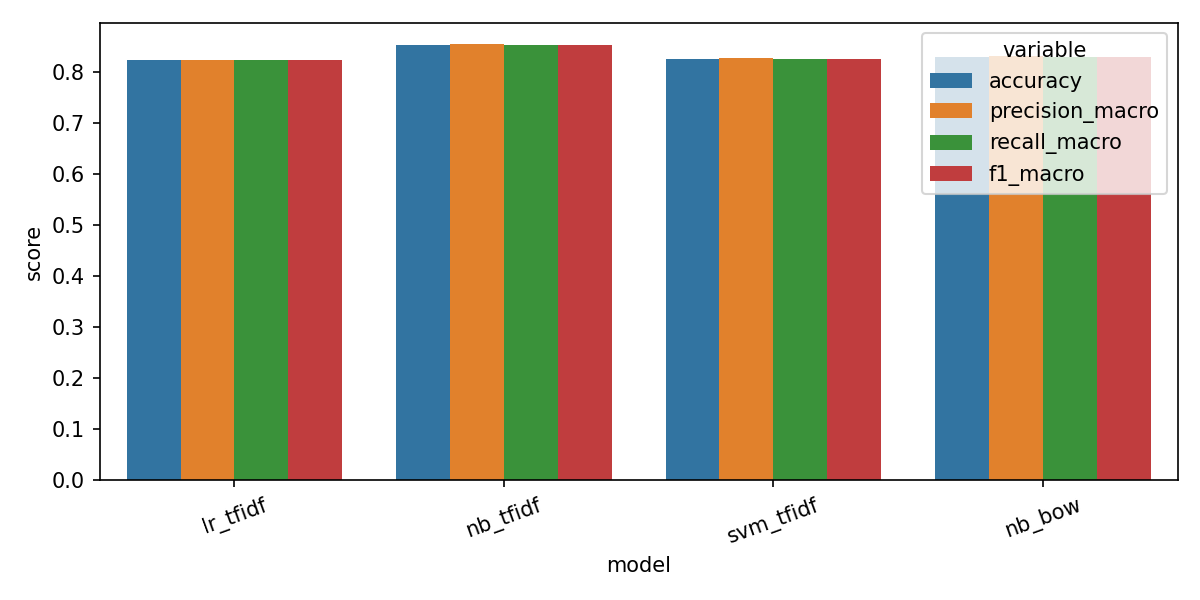
\includegraphics[width=0.82\linewidth]{figures/metrics_bar.png}
  \caption{Aggregate test-set metrics across the four pipelines. Multinomial Na\"ive Bayes on TF-IDF dominates every metric.}
  \label{fig:bar}
\end{figure}

\begin{figure}[ht]
  \centering
  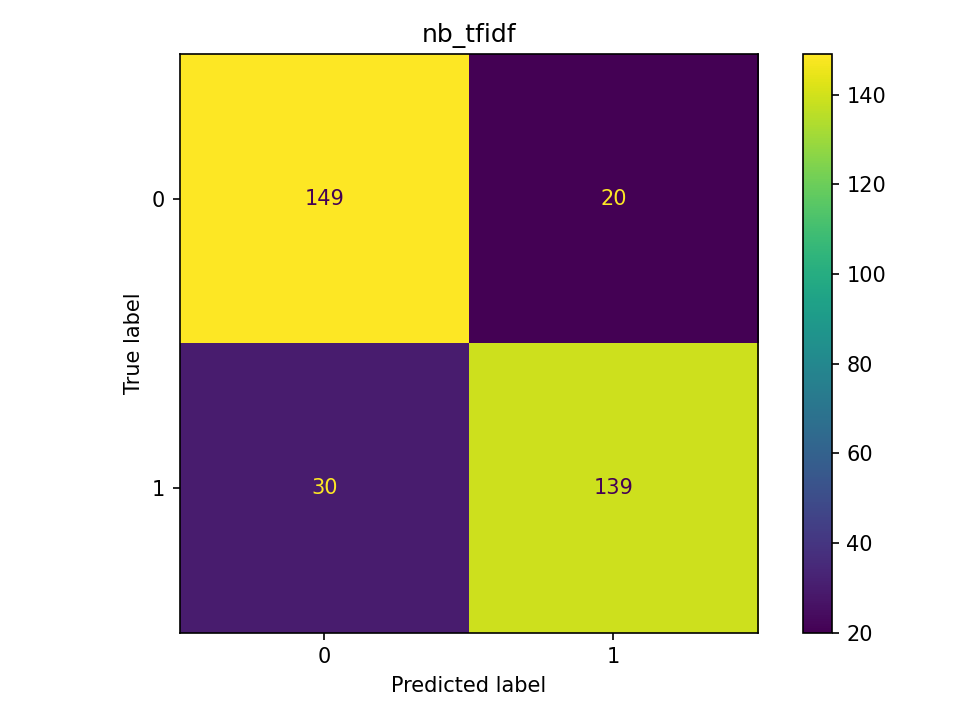
\includegraphics[width=0.55\linewidth]{figures/confusion_nb_tfidf.png}
  \caption{Confusion matrix for the best model (NB + TF-IDF). Errors are nearly symmetric between false positives and false negatives.}
  \label{fig:cm}
\end{figure}

\textbf{Interpretation.} The best model (NB + TF-IDF) reaches 0.852 test accuracy and 0.917 ROC AUC. Because the test set is exactly balanced, accuracy and macro F1 coincide and unambiguously summarise quality. The confusion matrix (Figure~\ref{fig:cm}) shows 149 true negatives, 20 false positives, 30 false negatives, and 139 true positives, i.e.\ the model leans very slightly toward the negative class. Practically, that means at the default threshold our errors are nearly symmetric; the high ROC AUC implies that, if the deployment scenario penalised one error type more than the other, threshold tuning could recover further targeted gains without retraining --- exactly the operating-curve argument made by~\citet{pang_lee_2008}.

\textbf{Comparison.} The most interesting finding is that NB + TF-IDF outperforms the two discriminative models by roughly three F1 points, and that NB + BoW is competitive with both LR and SVM. This is qualitatively the same conclusion reached by~\citet{wang_manning_2012}, who argue that ``NB does better than SVM for short snippet sentiment tasks''. Letterboxd reviews are not snippets, but the dataset is still relatively small (3{,}376 total examples after cleaning) and the bigrams give Na\"ive Bayes the local context it needs to be competitive. The two linear discriminative models (LR and SVM) finish within 0.003 of each other, which~\citet{joachims_1998} would expect because on sparse high-dimensional text, both linear losses converge to similar decision boundaries.

\textbf{Error analysis.} On the best model, 50 of 338 test examples ($\approx 14.8\%$) are misclassified. We exported all of them to \path{artifacts/error_analysis_samples.csv} and inspected the first 30 rows; five recurring failure modes account for the bulk of the errors (Table~\ref{tab:errors}).

\begin{table}[ht]
  \centering
  \footnotesize
  \caption{Representative misclassifications on the test set (best model, NB + TF-IDF). Snippets verbatim from \protect\path{artifacts/error_analysis_samples.csv}; long quotes truncated with `\dots'.}
  \label{tab:errors}
  \begin{tabularx}{\linewidth}{@{}cc>{\raggedright\arraybackslash}p{2.6cm}X@{}}
    \toprule
    True & Pred & Mode & Excerpt \\
    \midrule
    1 & 0 & Sarcastic praise & ``This movie is so good it's actually rather cringe.'' \\
    1 & 0 & Negative-sounding praise & ``Very few films have made me feel physically sick but this is one of them.'' \\
    0 & 1 & Backhanded compliment & ``Pointless film, but Daniel Day-Lewis gives an astonishing performance as Waluigi.'' \\
    0 & 1 & Praise of negative content & ``You can't show me the reality of war \dots Make up your mind. Is this brutal or is it John Wick?'' \\
    0 & 1 & Mixed sentiment & ``Rue Morgue CineMacabre Movie Night! Great FXs.'' (rated low overall). \\
    1 & 0 & Non-English text & ``$\delta\epsilon\nu$ $\tau o$ $\pi\iota\sigma\tau\epsilon\acute{\upsilon}\omega$\dots'' (Greek). \\
    \bottomrule
  \end{tabularx}
\end{table}

The patterns are exactly the ones~\citet{pang_lee_2008} catalogue as the hard cases for bag-of-words sentiment classifiers: sarcasm and contrast (\textit{``so good it's actually rather cringe''}) confuse models that discard word order; reviews that praise dark or violent content (\textit{``physically sick \dots one of them''}) are systematically read as negative because the surface vocabulary is negative; very short reviews give too few tokens for a confident posterior; and non-English tokens completely bypass our English vocabulary. Each of these is a known open problem in the classical literature, which is part of why~\citet{maas_imdb_2011} introduced learned word vectors and why~\citet{devlin_bert_2019} eventually replaced sparse features altogether.

\section{Conclusions}
\label{sec:conclude}

\textbf{Summary of findings.} The strongest classical pipeline on cleaned, balanced Letterboxd reviews is multinomial Na\"ive Bayes on TF-IDF unigrams and bigrams (accuracy 0.852, macro F1 0.852, ROC AUC 0.917). The two linear discriminative models cluster around 0.82 macro F1, and the bag-of-words ablation shows that TF-IDF weighting accounts for roughly two and a half F1 points of NB's advantage. Quantitatively this matches the body of work that argues classical models with sensible features remain hard to beat on small text-classification tasks~\citep{joachims_1998, mccallum_nigam_1998, wang_manning_2012}.

\textbf{Links to project objectives.} The original objective was a transparent, well-justified sentiment classifier suitable for a coursework rubric. We met that objective: each pipeline component (cleaning, preprocessing, vectoriser, classifier, evaluator) is implemented in roughly fifty lines of Python, the cleaning audit is logged numerically (Section~\ref{sec:cleaning}), the model space is small enough that the cross-validation choices are easy to defend, and the resulting feature weights are inspectable n-grams.

\textbf{Limitations.} (i) Star-derived labels are noisy: the error analysis suggests several misclassifications are reviews whose prose genuinely disagrees with the star rating, exactly the issue~\citet{pang_lee_vaithyanathan_2002} flag for any rating-derived supervision signal. (ii) The Top-250 cut over-represents acclaimed films, narrowing the negative-vocabulary distribution. (iii) Bag-of-words style features cannot model negation, sarcasm, or long-range structure, all of which appear in our error table. (iv) Non-English reviews are out of scope of an English stopword list and an English lemmatiser, which causes systematic errors.

\textbf{Meaningful future improvements.} (i) Train on the unrestricted 90k export plus the companion ``Worst 250'' dataset to widen the negative-vocabulary distribution. (ii) Add a neutral class for 2.5--3.5-star reviews so the model can express genuine uncertainty rather than being forced to a binary call --- this is the same three-way framing used by~\citet{pang_lee_vaithyanathan_2002}. (iii) Replace the sparse vectoriser with pretrained word embeddings such as Word2Vec~\citep{mikolov_2013} or sentence embeddings derived from a small transformer (DistilBERT, following~\citet{devlin_bert_2019} and the protocol of~\citet{maas_imdb_2011}) to compare against a stronger upper bound. (iv) Add a language-identification pre-filter and route non-English reviews to a multilingual encoder. (v) Calibrate decision thresholds explicitly for asymmetric error costs.

\textbf{Reflection on challenges.} The two notable engineering wrinkles were (a) parsing the dataset's Unicode star encoding, which silently fails when treated as numeric and almost cost us our entire label set; and (b) the very strong positive class skew of the Top-250 cut, which forced us to redesign the balancing rule from ``cap each class at $N$'' to ``cap both classes at the smaller class count''. Both issues are now caught at load time and reported in the cleaning audit, which is exactly the discipline~\citet{pang_lee_2008} advocate when working with star-derived sentiment labels.

\bibliographystyle{plainnat}
\bibliography{references}

\end{document}
